\problemname{Danger Zone}

\illustration{0.4}{tables}{The round tables outside the university shop.}%
Will today be the day? Weeks have gone by and you barely remember the last time
you were lucky enough to get some candy at the university. All because of those
vicious round tables that surround the entrance to the shop, waiting for the
next absentminded student to wander into their midst, and hurt themselves by
walking into or tripping over one of the tables. ``\textit{I'm just going to
the shop to grab some treats}'' are the words of dozens of students never to be
seen again.

You silently observe the tables from a distance and look at the shop entrance
behind them with longing eyes. Maybe it's the current arrangement of the round
tables, but you feel like --- with a good plan --- today might be the day you
finally manage to navigate around the round tables to the entrance of the shop,
and get your oh-so-wanted candy.

\begin{figure}[h!]
  \centering
  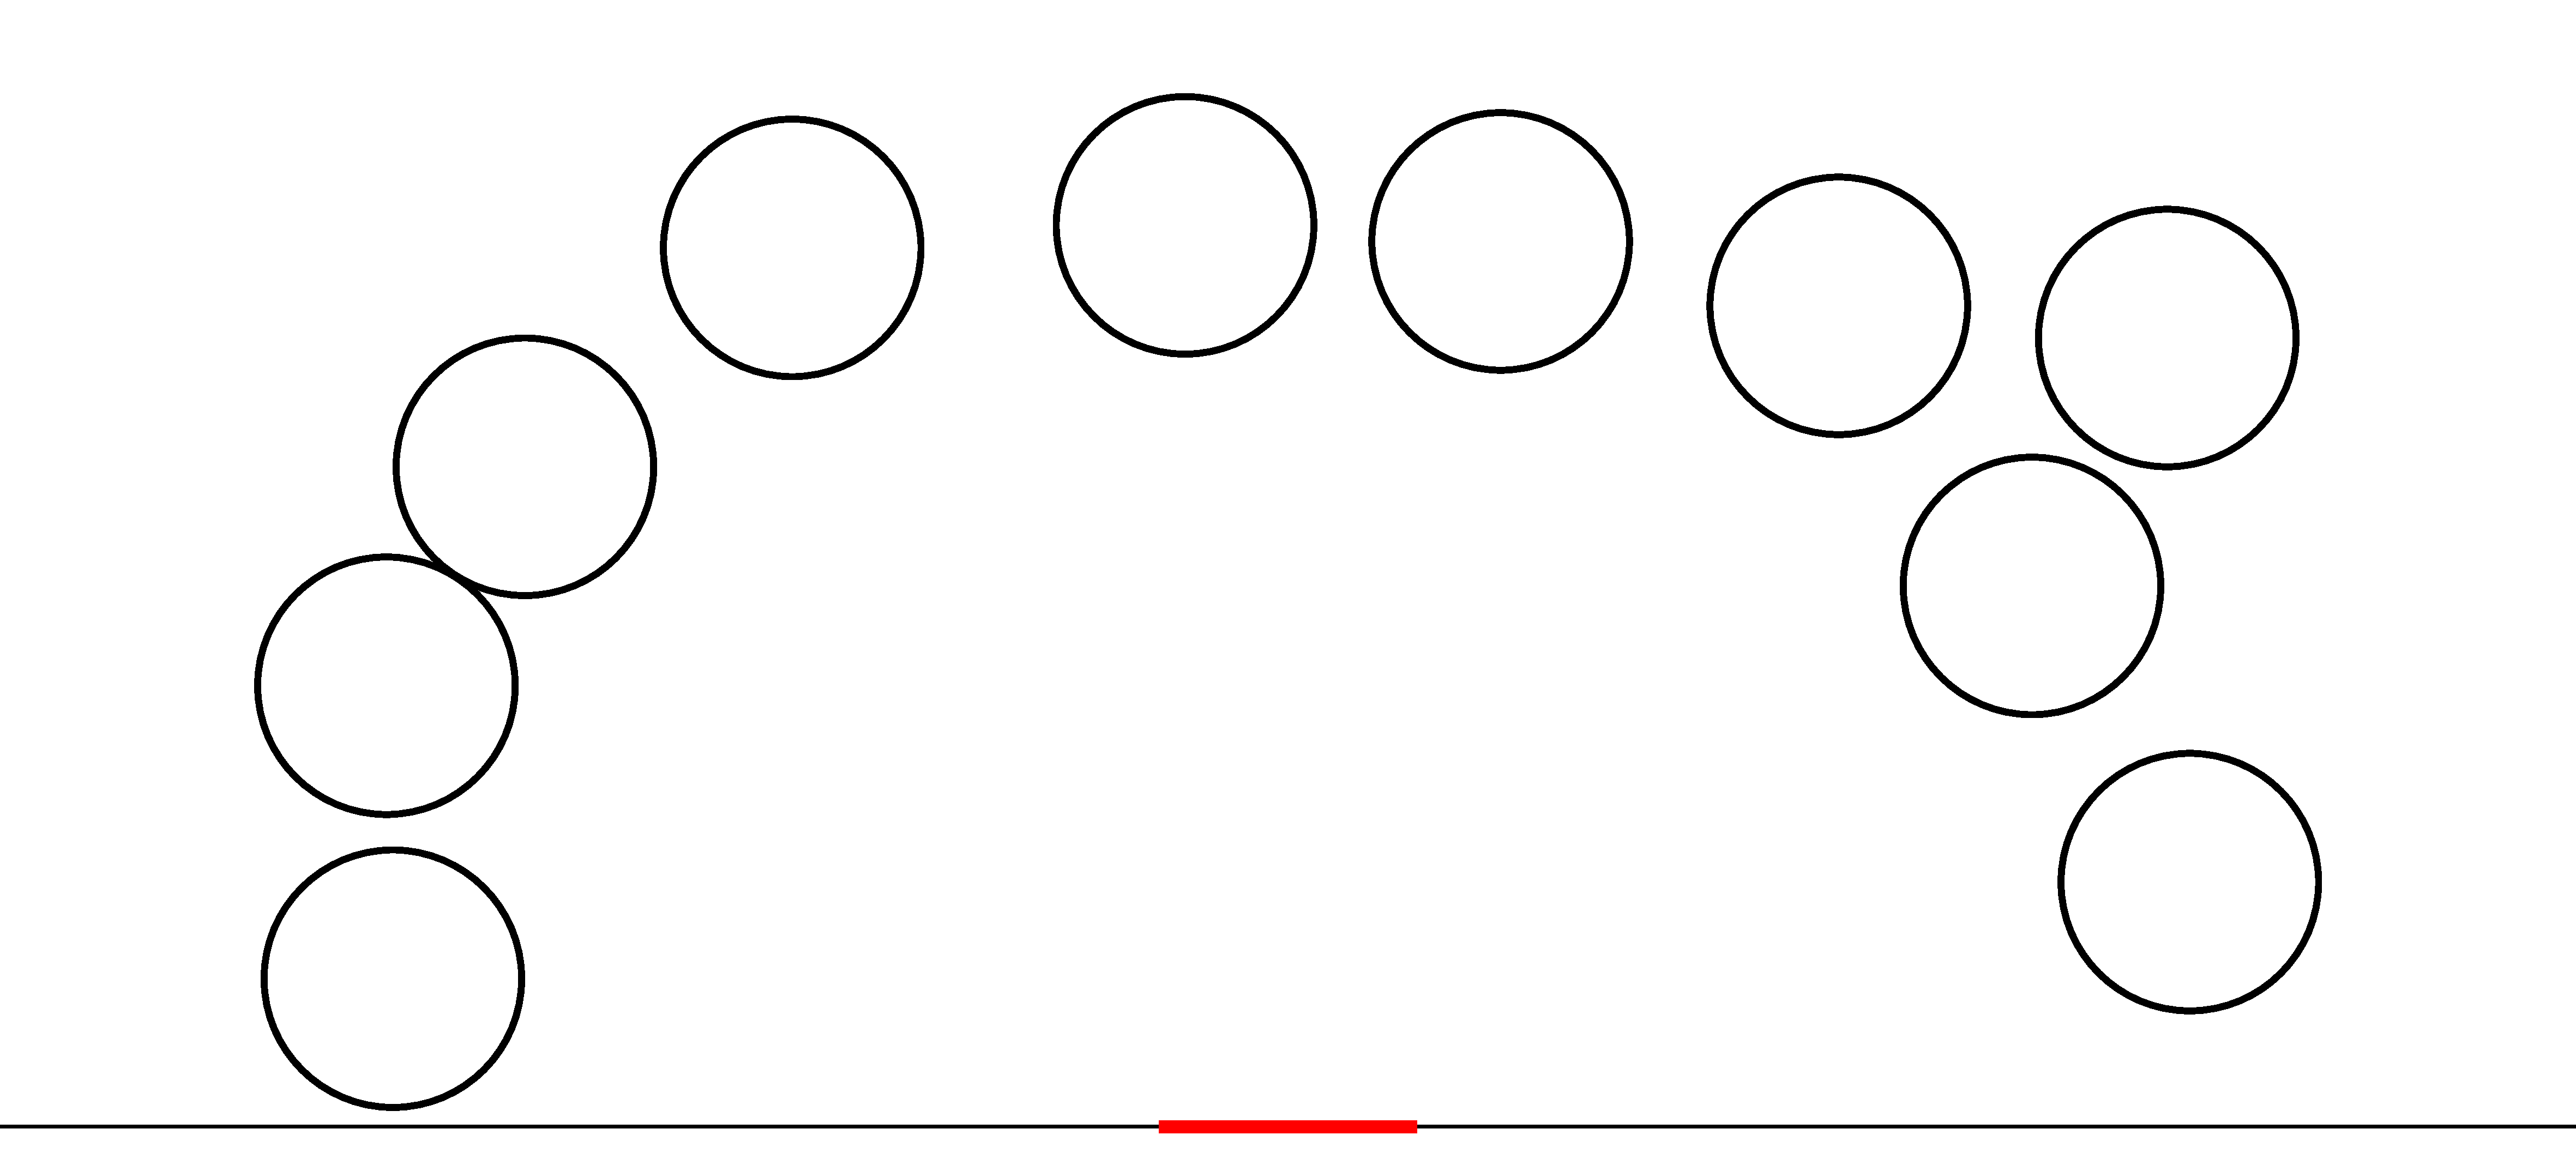
\includegraphics[width=0.70\textwidth]{figure}
  \caption{Illustration of Sample Input 2, with the entrance to the shop in red.}%
  \label{fig:sample2}
\end{figure}

The round tables are represented as a set of non-intersecting circles, each of
diameter $80$ centimetres. The front of the shop is represented as the infinite
$x$-axis facing the positive $y$ direction. The entrance to the shop is
represented as a line segment on the $x$-axis, with midpoint $(0,0)$ and length
$80$ centimetres. You are represented as a circle of diameter $50$ centimetres.
Although you can touch the front of the shop and the edges of the tables, you
cannot walk through walls and you will certainly not climb over or under the
tables. You're not willing to take any such chances!

Given the locations of the tables in centimetres relative to the midpoint of
the shop entrance, can you navigate past the tables and reach the entrance?
You are currently far enough from the entrance that your precise location is
irrelevant.

\section*{Input}
The input consists of:
\begin{itemize}
    \item One line with one integer $n$ ($0 \le n \le 5\,000$), the number of round tables.
    \item $n$ lines, the $i$th of which contains two integers $x_i$ and $y_i$
    ($|x_i| \le 10^9$, $40 \le y_i \le 10^9$), the location of the
    center of the $i$th round table in centimetres relative to the midpoint of
    the shop entrance.
\end{itemize}

No two tables intersect, and each table is at least $2$ metres away from the
shop entrance.

\section*{Output}
Output ``\texttt{possible}'' if it is possible to reach the entrance. Otherwise
output ``\texttt{impossible}''.

